


\section{Section 1: Smart metering}

In this section, special attention is given to smart metering. The smart grid framework is presented to justify the need for smart meters and then, an overview on metering systems is presented.


1.	Smart grids and the need for smart meters

2.	Metering systems – overview

3.	Metering systems in railways

4.	Wireless sensor networks – overview

5.	Smart metering with WSN in Railway Transportation System (RTS)

\subsection{Smart grids and the need for smart meters}

Smart Grids improves the functionality and concept of traditional electrical grids by obtaining the grid component's data using Information and Communication Technology (ICT). Such grids benefit the reliability and the efficiency of the system with the usage of the acquired data, \cite{Mohassel2014}.

Although the smart meters does not have an effective definition, those devices are composed by an electronic box and a communication link, \cite{Seppo2012}. A smart meter is responsible for measuring the energy-related parameters and the user consumption with a given time interval. All those measurements are then transmitted upon a communication network to the utility or to other player with the responsibility of using the meter data. The information obtained from the data is shared with consumer-side devices, to inform the end-users on their related costs and energy usage, \cite{Siano2014}.

Smart meters implement a bidirectional communication on top of AMR. They are inherent to smart grid systems. 

Similarly to the evolution of electricity meters, the utility grid has evolved from a centralized production and control perspective to a distributed one. The conventional electrical grid is a network with a transmission link connecting power producers and end-user consumers. The control and distribution of electrical power is made in a centralized way. With the increase of power demand, increase of complexity and having more and more decentralized power generation, a migration to the smart grid framework is required, \cite{Reddy2014}.

\subsection{Features of Smart Meters and metering systems}

A smart metering system combines several controlling devices, a extensive number of sensors for measuring the parameters and devices responsible for the transferring of the data and the commands. The detection of unauthorized consumption due to electrical energy theft and the improvement of the energy in the distribution are other advantages of smart meters. These devices acts as a gateway by having a communication interface protocol to the database stored by the utility company, \cite{Reddy2014}.

The design of an ideal smart grid has to focus on prediction, adaptability and reliability points. Moreover, it requires to cover the demand adjustment, the load handling, flexibility and sustainability and it should incorporate advanced services. In advance, an end to end control capability has to be ensured as well as finding the optimal cost and asses, increase the quality of energy and quality of service. Another features of smart grids are the automatic restoration ans self-healing, being all the previously presented features of the smart grids highly dependent of the role of the smart meters, \cite{Mohassel2014}.

Smart-meter types are also distinguished based on features like data-storage, communication type and connection with the energy supplier. The data storage capability allows data to be stored in the meter, being transferred after a few days or weeks to the Meter Data Management System (MDMS) of the utility. Compensations for some power quality deficiencies can be also considered; therefore the future meters should be also capable of register certain basic power quality characteristics. In advance, the design of rate and tariffs of electricity providers determine the requirements such as the period of meter intervals or the temporal resolution (commonly ranging from 15 min to 1 h). During those intervals, the production and consumption of active and reactive power is mandatory to be separately measured, \cite{Siano2014}.

\subsection{Metering systems in railways}

Towards na increase of interoperability of the rail system within the Community \cite{eur-lex2008}, the Directive 2008/57/EC specifies the need of Technical Specifications for Interoperability (TSIs), presenting essential requirements in which each rail subsystem should meet to ensure the interoperability of the railway system within the EU. Those TSIs are of the responsibility of European Union Agency for Railways (ERA) and are listed as following:

\begin{itemize}
	\setlength\itemsep{-0.5em}
	\item Locomotives and passenger rolling stock - 1302/2014;
	\item Noise - 1304/2014;
	\item Wagons - 321/2013;
	\item Infrastructure - 1299/2014/EU;
	\item Energy - 1301/2014;
	\item Control command and signalling - 2012/88/EU;
	\item Persons with reduced mobility - 1300/2014/EU;
	\item Safety in railway tunnels - 1303/2014;
	\item Operation and traffic management - 2015/995/EU;
	\item Telematics applications for freight service - 1305/2014/EU;
	\item Telematics applications for passenger service - 454/2011;
		
\end{itemize}


On the energy field and with the purpose of implementing on-ground energy data collecting systems (data collecting service - DCS), technical specifications for interoperability relating to the ‘energy’ subsystem of the rail system in the Union are specified in the Commission Regulation (EU) No 1301/2014, \cite{eur-lex2014}. 



The On-Board energy measurement systems are pointed in Appendix D of Commission Regulation (EU) No 1302/2014 \cite{eur-lex2014b}. This regulation appendix presents the requirements for such energy measurement system. The general architecture is defined as following:

\begin{itemize}
	\setlength\itemsep{-0.5em}
	\item \textbf{Energy measurement function (EMF)}, measuring the voltage and current, calculating the energy and producing energy data;
	\item \textbf{Data handling system (DHS)}, producing compiled energy billing data sets for energy billing purposes, by merging data from the EMF with time data and geographical position, and storing it to be sent to on-ground data collection system (DCS) by a communication system;
	\item \textbf{On-board location function}, giving geographical position of the traction unit. Contrary to fixed installation revenue meters, train meters must have the knowledge of time and geographical position \cite{metas2015};
\end{itemize}

Figure \ref{fig:EMS} presents the general overview of the on-board energy measurement system.

\begin{figure}[h!]
	\centering
	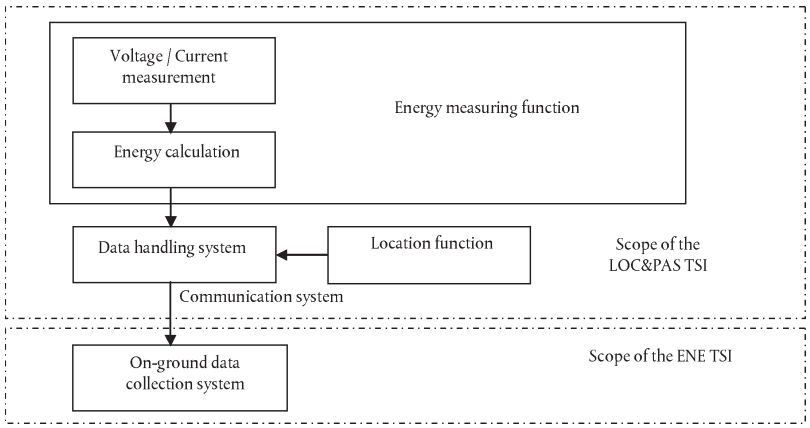
\includegraphics[width=0.85\textwidth,keepaspectratio]{figures/EMS}
	\caption{Functions, data flow and regulation scope of on-board energy measurement system.}
	\label{fig:EMS}
\end{figure}

As global requirements, all active and reactive energy should be measured, the measurement equipments should be rated to match the traction unit current and voltage rating, the system should be protected from intrusion, and finally, the loss of power in the  measurement system should not affect the data stored in EMS.

Complementary to the previously presented system requirements, each component of the energy measurement system has specific requirements as listed as following:

\begin{description}
	\setlength\itemsep{-0.5em}
	
	\item [Energy measurement function (EMF)] Has specific metrological requirements to specify the accuracy of the sensors and it has the requirement of having the reference period of 5 minutes defined by the UTC clock time (shorter measuring period is allowed in the case that the data is aggregated into 5 minutes time reference period);
	
	\item [Data handling system (DHS)] Should compile the data (without corrupting them), using the same time reference as EMF. This system should store compiled data of, at least, 60 days' continuous work and should have an alternative method of accessing the data. Finally, this system should produce compiled energy billing data sets (CEBD) by including an EMS identification number, a timestamp, a location data and the consumed/regenerated active and reactive energy.
	
	\item [Location function] Has specific location requirements to define the latitude and longitude, as well as a accuracy of 250m and the location data information should have the same timestamp.
	
	\item [On-board to ground communication] The specification related to interface protocols and transferred data format are an open point.
	
\end{description} 


 \cite{metas2015} lists the standards that should be considered to the certification of Energy Measurement Systems on on-board trains:
 
 \begin{description}
 	\setlength\itemsep{-0.5em}
	\item [EN 50463-1] General;
	\item [EN 50463-3] Data Handling System;
	\item [EN 50463-4] Communication;
	\item [EN 50463-5] Conformity Assessment.
 \end{description} 




%\subsection{Wireless sensor networks – overview}


\subsection{Smart metering with WSN in Railway Transportation System (RTS)}


%%%%%%%%%%%%%%%%%%%%%%%%%%%%%%%%
%%%%%%%%%%%%%%%%%%%%%%%%%%%%%%%%%
%%%%%%%%%%%%%%%%%%%%%%%%%%%%%%%%%